The observation of the first multiply-imaged, gravitationally lensed supernova (SN) in 2014, SN ``Refsdal", 
was a critical step forward in the SN cosmology community (Figure 1; \citet{Kelly:2015a}). The scientific
merit of correctly analyzing multiply-imaged SNe is well known, as accurate measurements of time delays and magnification ratios
can provide valuable constraints on $H_0$, yield powerful new estimates of dark energy parameters, and deliver a unique test of 
systematic biases in other cosmological probes (\citet{Jha:2007},\citet{Treu:2013}). While early work did estimate these parameters, 
the considerable benefits of such results warrant efforts at improving the precision reached in the initial measurements. Therefore, 
we propose to perform a comprehensive reanalysis of SN Refsdal in order to refine our constraints on the lensing parameters. 
We will improve upon previous work by making substantial improvements to the photometry, and including 
the significant yet previously ignored effects of microlensing. Additionally, we will produce an open-source software 
package in the course of this work, optimized specifically for multiply-imaged SNe. Therefore, we will not only produce 
valuable science by increasing the precision of SN Refsdal lensing measurements, but will also provide JWST/LSST era astronomers 
with a thorough methodology and a critical tool to analyze the expected dramatic increase in lensed SNe.


\begin{figure}[h]
\centering
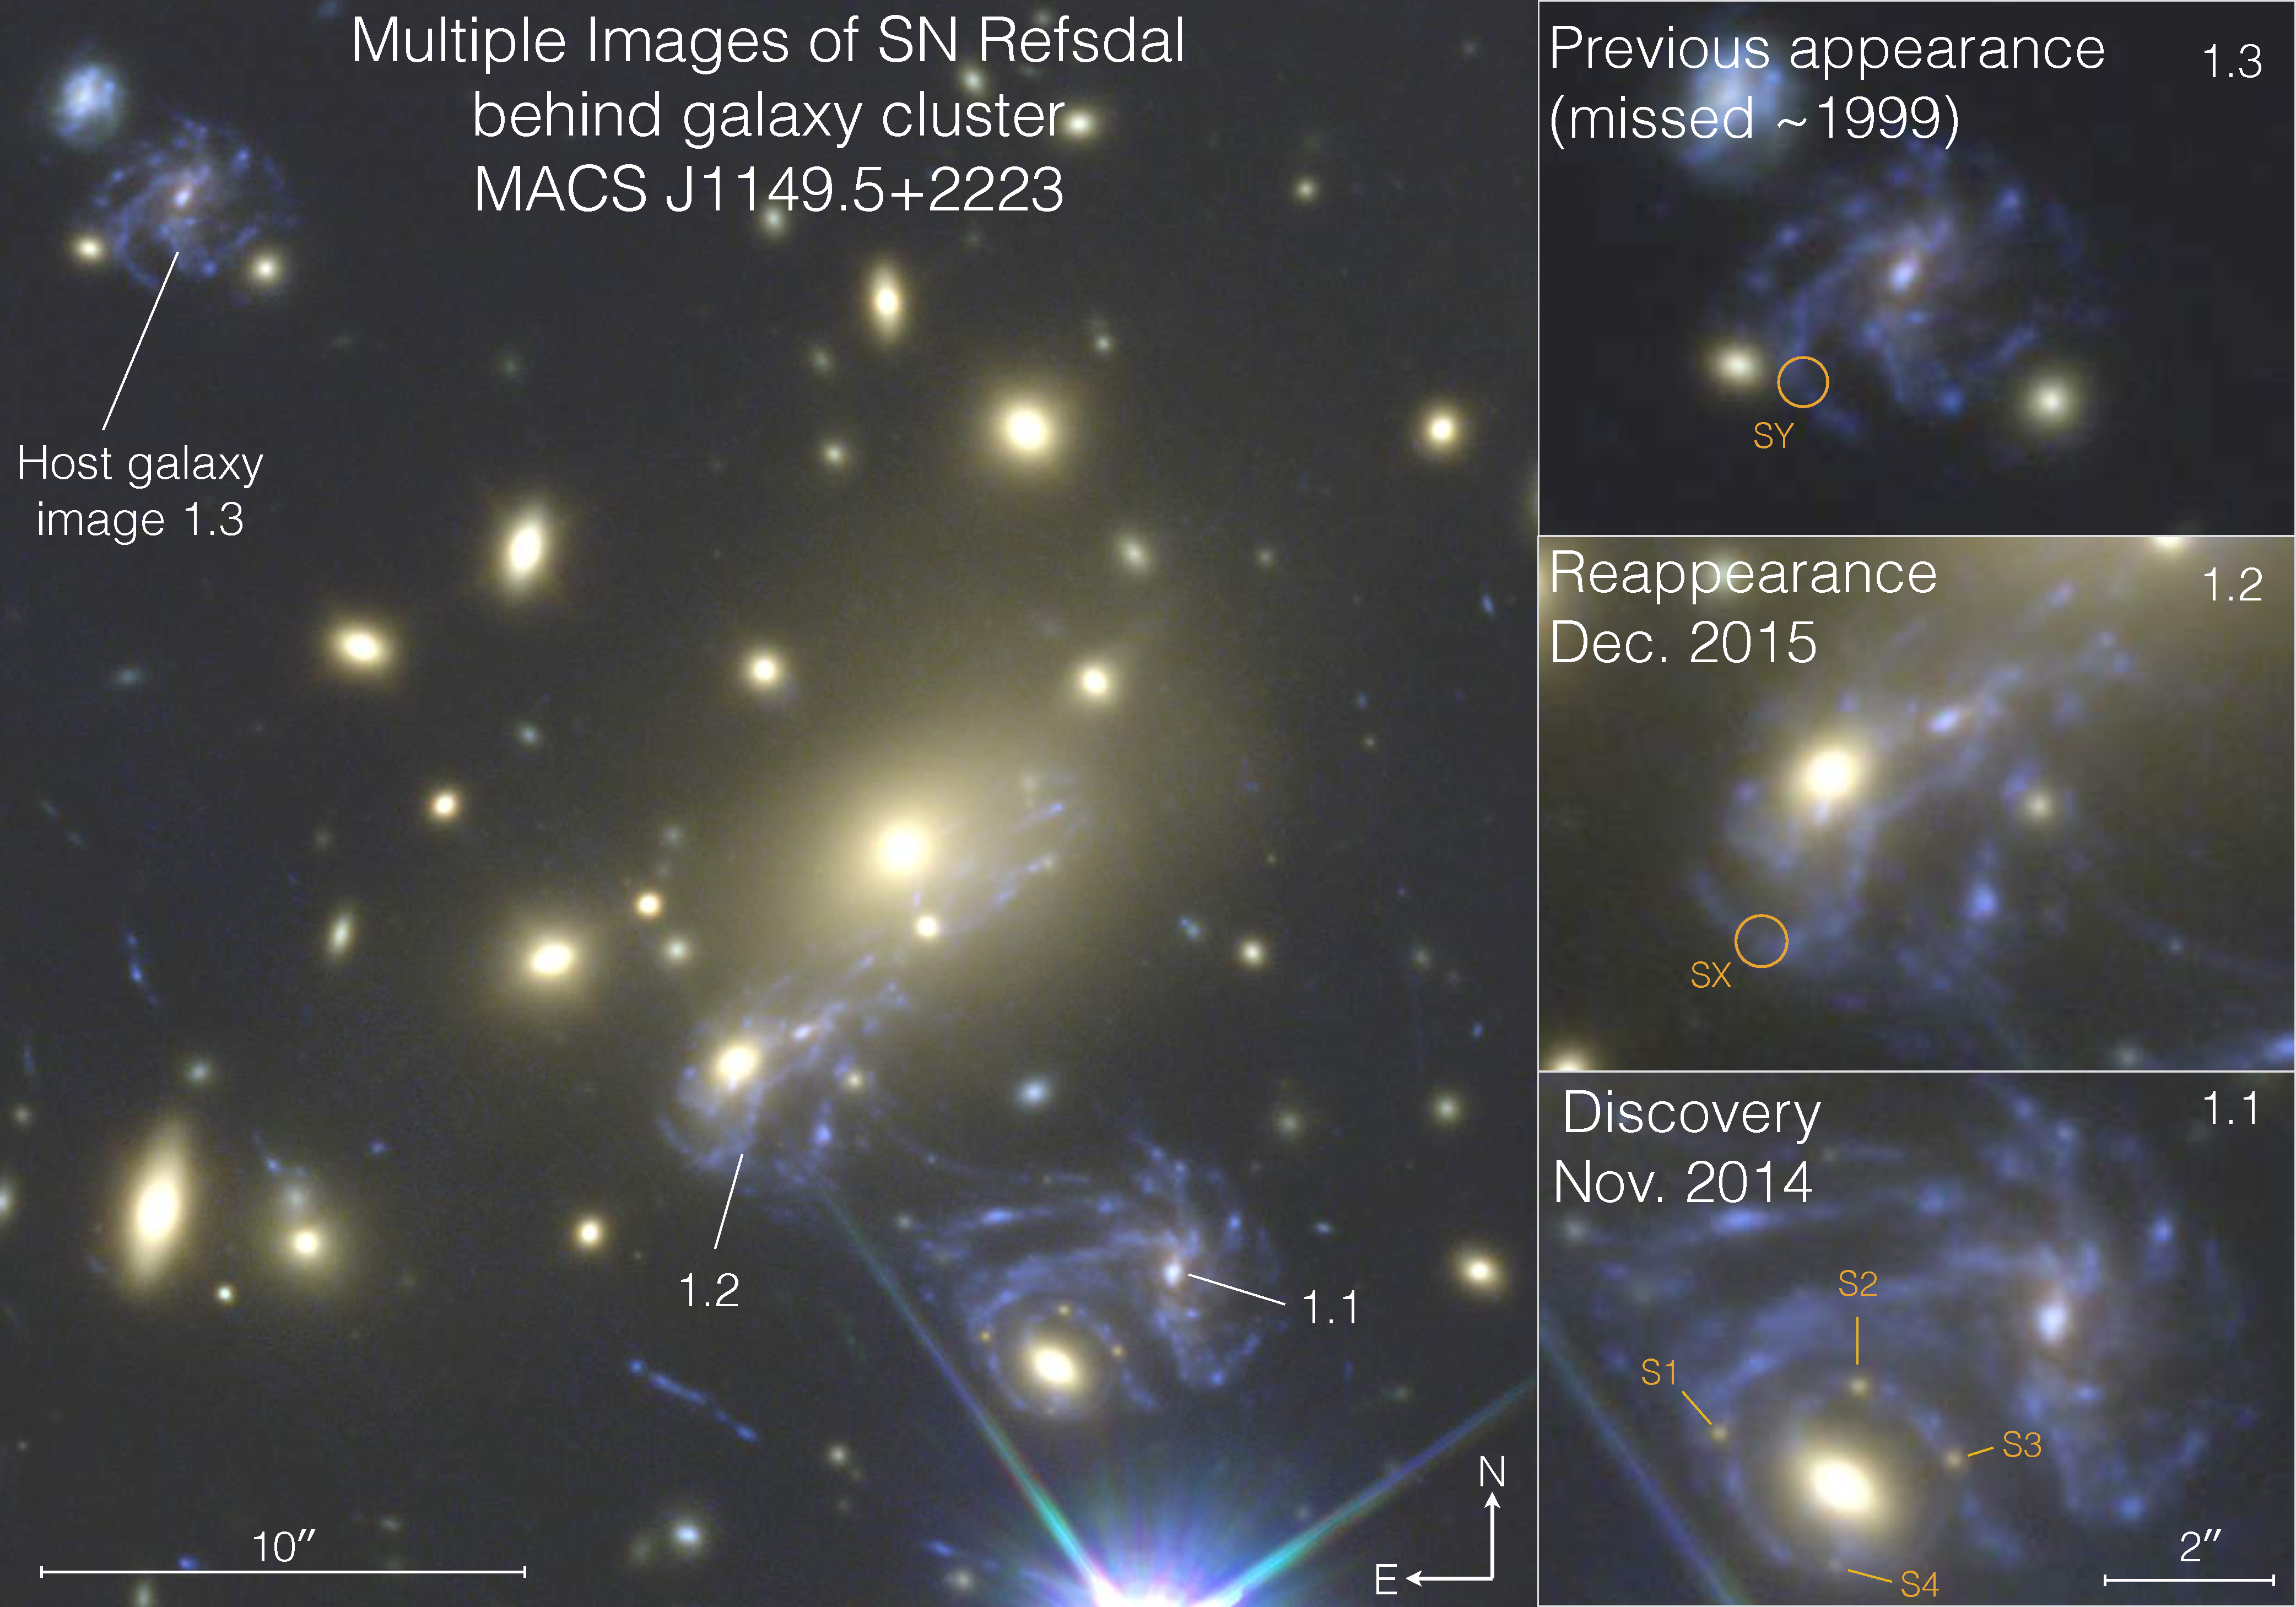
\includegraphics[width=0.8\textwidth]{FIG/refsdal_rodney.pdf}
\caption{
MACS J1149.6+2223 field, showing the positions of the three primary
images of the SN Refsdal host galaxy (labeled 1.1, 1.2, and 1.3). SN
Refsdal appears as four point sources in an Einstein Cross
configuration in the southeast spiral arm of image 1.1 \citep{Rodney:2016}}
\end{figure}

\pagebreak

\noindent {\bf Time Delay Cosmography:}

\

\begin{figure}[h]
\centering
\vspace{-1em}
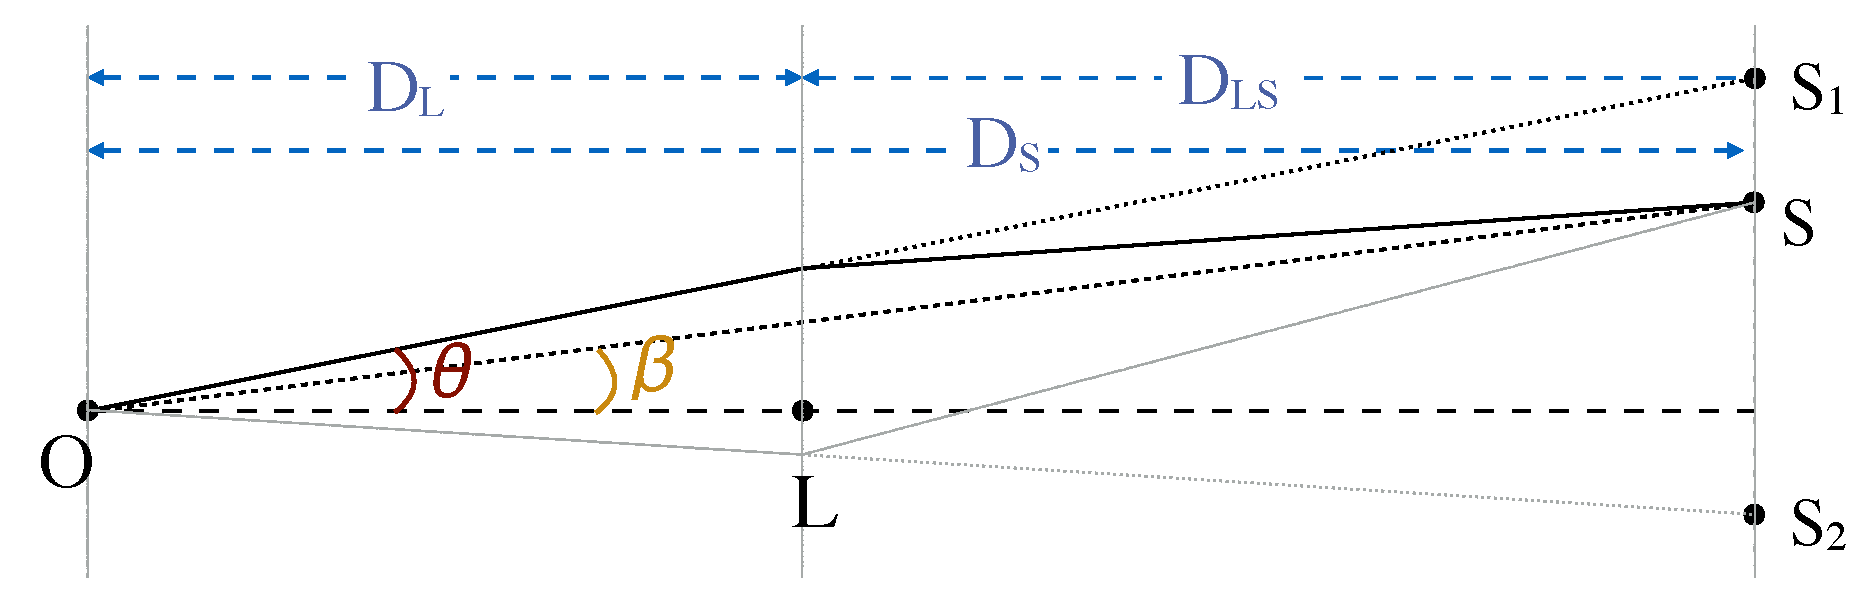
\includegraphics[width=.7\textwidth]{FIG/lensingGeometry2}
\end{figure}

As light from a distant
source passes through a gravitational lens, each subsequent image will appear to the observer delayed by 


\begin{equation}\label{eq:dt}
  \dt = \frac{(1+z_L)}{c}\frac{\Dl \Ds}{\,\Dls} \left(\frac{1}{2}(\theta-\beta)^2 - \psi(\theta)\right)
\end{equation}

\noindent (relative to the unlensed travel time). Here, $z_L$ is the redshift of the lens, while \Dl, \Ds, 
and \Dls\ are angular diamater distances from the observer to the
lens, observer to source, and lens to source, respectively.  The time
delay has a geometric component due to light rays following different
path lengths to the observer, plus a general relativistic component,
$\psi$, due to differing values of the gravitational potential along
each path. The distance ratio $\Dl\Ds/\Dls$ in Eq.~\ref{eq:dt} carries
a factor \Ho$^{-1}$, so if the lensing potential $\psi$ is well known,
then the {\bf time delay measurement  provides a direct constraint on
the Hubble constant that is completely independent of the local distance
ladder.}

\bigskip

\noindent {\bf A New Software Package:}

\

In addition to the first discovered multiply-imaged SN (Refsdal), a lensed Type 1a SN was found
by \cite{Goobar:2016}, and \textbf{the next decade is expected to yield observations
of over 100 lensed SNe} that will require analysis \citep{Oguri:2010}.
To date, \textbf{there is no public software package for analyzing multiply-imaged SNe.}
The lack of a standard resource leaves researchers to write and implement their 
own ad hoc programs, which will become increasingly inefficient as the number of
observed lensed SNe increases. An optimized software package with the ability to fully 
analyze a light curve and rigorously include the effects of gravitational lensing would be extremely valuable to a wide range of
research using current and next generation telescopes. In the course of completing this work, 
we are producing an open-source software package written in Python for use in this and future SN analysis. This package will
lead to an \textbf{improved understanding of the complex effects acting on 
multiply-imaged SNe}, as well as provide a \textbf{standard tool} for future use in the SN cosmology 
research community.

There are currently two software packages that form the basis 
of this product: Python Curve Shifting (PyCS) used for quasars, and Supernova Cosmology 
(SNCosmo). First, these two packages will be integrated, giving researchers a tool
that can model SN light curve data with the abilities present in either
software package. Second, we will extend and optimize the quasar lensing and microlensing
algorithm present in PyCS for SNe, which is an essential step in acquiring accurate measurements
of multiply-imaged SN time delays and magnification ratios. Unlike quasars, SNe of a given class 
always have consistent and well-known light curve shapes. This will allow for physically motivated, 
less flexible models that will be more likely than PyCS to correctly identify SN 
microlensing effects and produce simpler time delay measurements. By allowing certain constraints to float as free 
parameters, these models will also produce best-fit synthetic light curves from which time delays, magnifications, 
SN class, and redshift can be derived. By simulating large numbers of SNe with these synthetic light curves, we will 
be able to quantify the accuracy and efficiency of the software.
\bigskip

\noindent {\bf Microlensing Effects:}

\

Microlensing refers to the small-scale gravitational lensing
perturbations due to massive objects along the light path of any one image of a
multiply-imaged SN. The effect of microlensing is to cause distortions in the SN light
curves that significantly limit the precision that can be achieved in the measurement of 
their time delays. After the discovery of Refsdal in 2014, subsequent work was done to 
classify the SN \citep{Kelly:2016}, as well as measure time delays and magnification
ratios \citep{Rodney:2016}. However, throughout the previous analyses the effects of 
microlensing were completely ignored. Therefore, this work will \textbf{fully analyze the effects
of microlensing on a multiply-imaged SN for the first time.}

There are two types of microlensing to consider in this reanalysis. The first is currently
considered in quasar time delay measurements and is caused by transverse motion 
of stars in the lensing galaxy (type 1). The second form (type 2) develops when the 
expanding photosphere of a SN interacts with an increasing volume of the caustic web, 
precipitating microlensing effects described by \cite{Dobler:2006} that can cause 
fluctuations of $\sim$0.2 to $>$0.5 magnitude on timescales of weeks to months. Type 2
microlensing is unique to lensed SNe, and has therefore never been fully classified or considered in lensed SN
analysis: In preparing this proposal, we have already used flexible functions to preliminarily measure the
effects of the type 1 microlensing (Figure 2), and it's clear that microlensing must be taken into account in order
to ensure accurate time delay and magnification measurements. While tools currently exist that utilize 
flexible polynomials to measure the effects of type 1 microlensing on quasars, no software package 
currently exists capable of considering the type 2 microlensing effects unique to lensed SNe. 
Therefore, the algorithm will be developed following the methodology of \cite{Dobler:2006} and released 
as a component of the open-source software packaged being developed in the course of this work. 

\pagebreak

\begin{figure}[H]
\centering
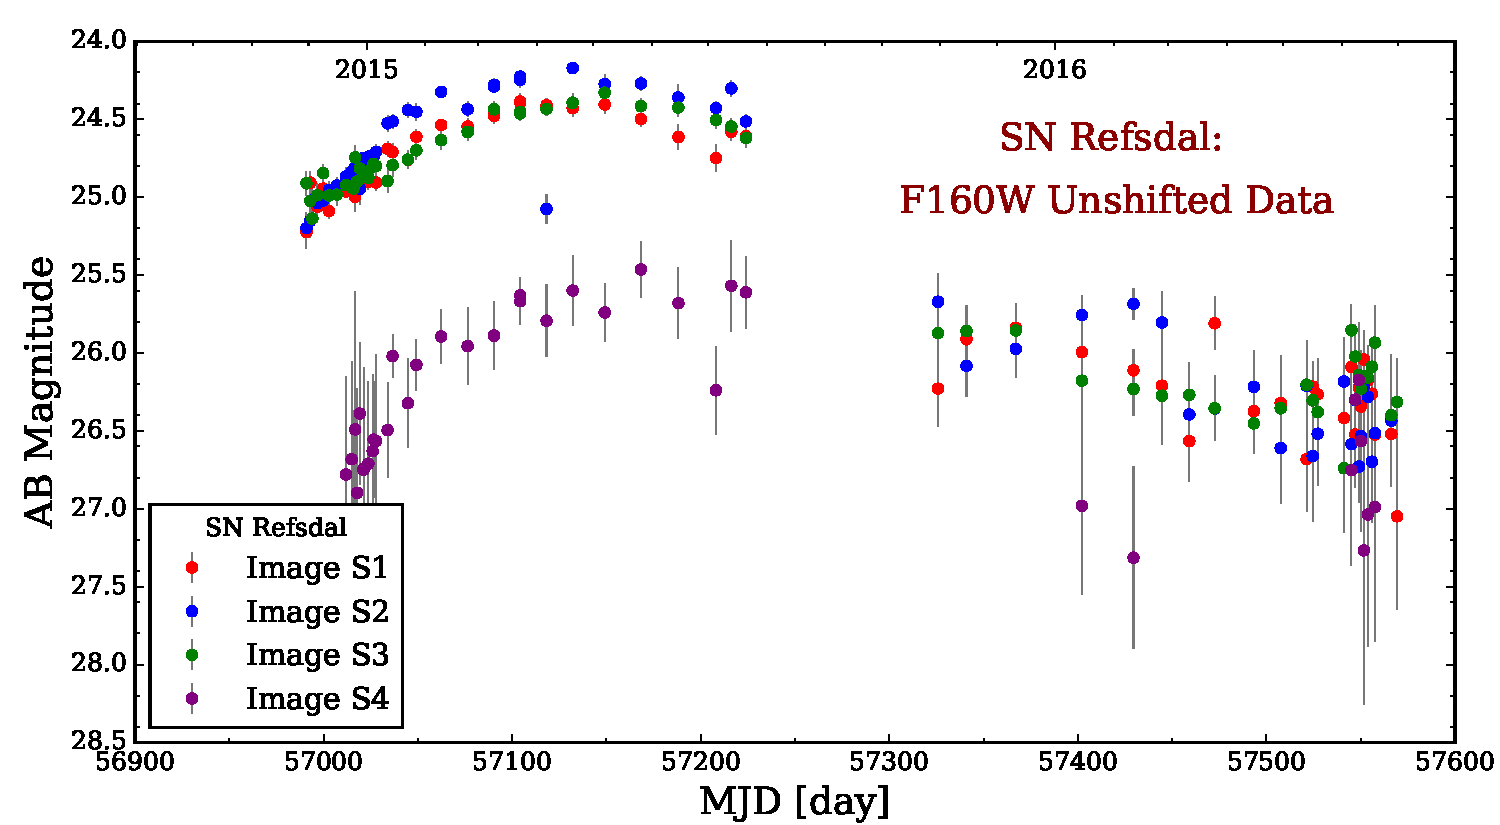
\includegraphics[width=.7\textwidth]{FIG/points_plot_2017.pdf}
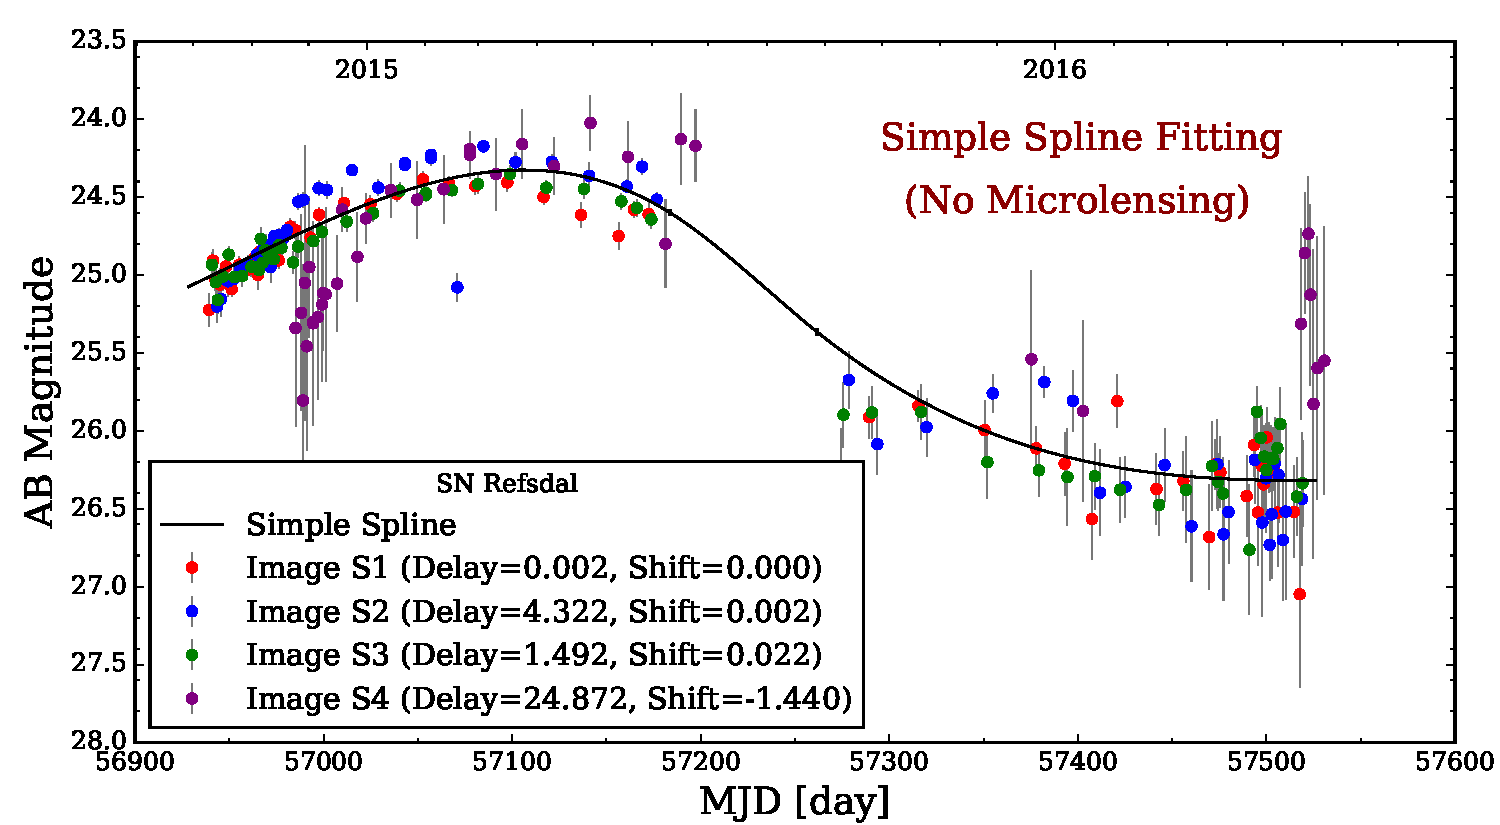
\includegraphics[width=.7\textwidth]{FIG/refs_plot_2017.pdf}
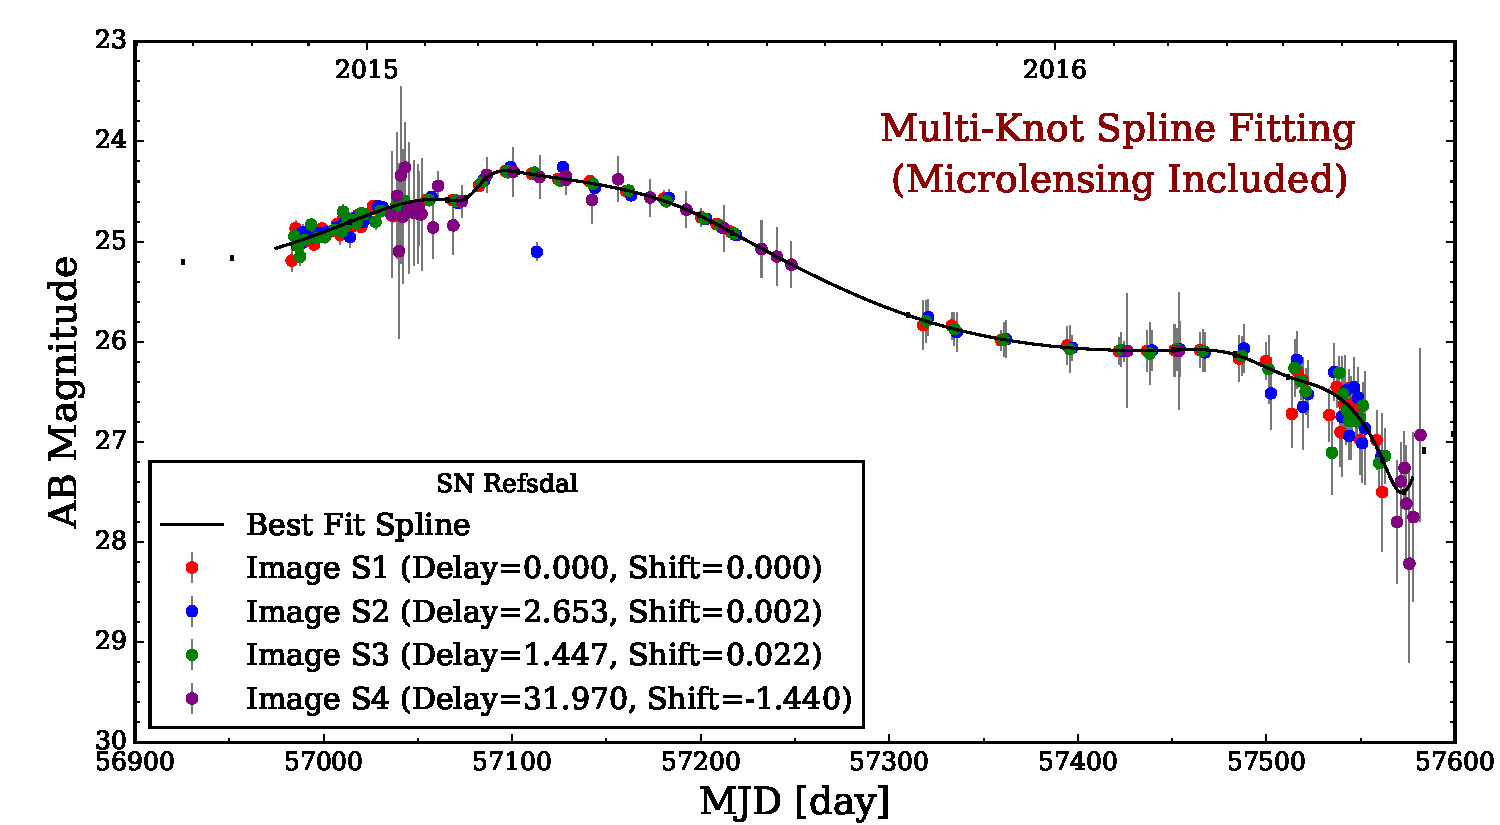
\includegraphics[width=.7\textwidth]{FIG/spline_plot_2017.pdf}
\caption{(Top) HST F160W data representing the four images of SN
Refsdal (Figure 1), with no lensing or time shifts. (Middle) Method of
fitting the SN Refsdal light curves from Rodney et al. 2016, which did
not consider microlensing effects. (Bottom) Preliminary results from 
this work using a multi-knot spline to fit the data. This method 
includes microlensing effects, which leads to a slight adjustment in 
time delay measurements. }
\end{figure}

\bigskip

\noindent {\bf Improving Photometry:}

\

Ensuring accurate photometry is an essential component of an accurate measurement of time delays for a multiply-imaged SN. 
The python software package \textit{PythonPhot} \citep{Jones:2015} was used for photometric measurements in the initial analysis
\citep{Rodney:2016}, but the use of a single photometric tool means that potential systematic errors may be disregarded. 
As a check against systematic biases, our reanalysis will use both the \textit{PythonPhot} and the \textit{DOLPHOT} package to 
measure photometry. We will also measure the photometry in single-exposure images, allowing us to check for any deviations 
at very short timescales, indicative of very rapid microlensing events. \cite{Rodney:2016} measured flux using a single empirical 
point-spread function (PSF) fixed in time, derived from standard stars. However, as we know that the HST PSF does undergo 
subtle variations due to telescope ``breathing" (cite), our re-analysis will use foreground stars within the MACS1149 imaging 
datasets to define a variable PSF model. \textbf{The reduction of systematic biases in the photometry and our improvements to the 
PSF will provide drastically ameliorated flux calculations, which in turn will increase the accuracy and precision of time delay 
measurements in our reanalysis.}




